\subsection{Test Case Descriptions \& Raw DecaWave Data}

The raw DecaWave data is shown in Figure~\ref{figure:decawave123_raw}.
During tests 1 and 3, the data collection platform moved from $(x,y)\approx(5,1.8)$
to $(x,y)\approx(12.5,15)$ along an L-shaped path with a single clockwise $90^\circ$ turn.
During test 2, the drone followed the same path in the opposite direction.
This most positional variance appears in the top left of the path, where the path is both
near to a wall and to the wall of the convex hull bounding the anchors for the DecaWave system.
Test 1 is representative of the other 2 tests, and they have therefore been left for conciseness.

\begin{figure}[h]
     \centering
         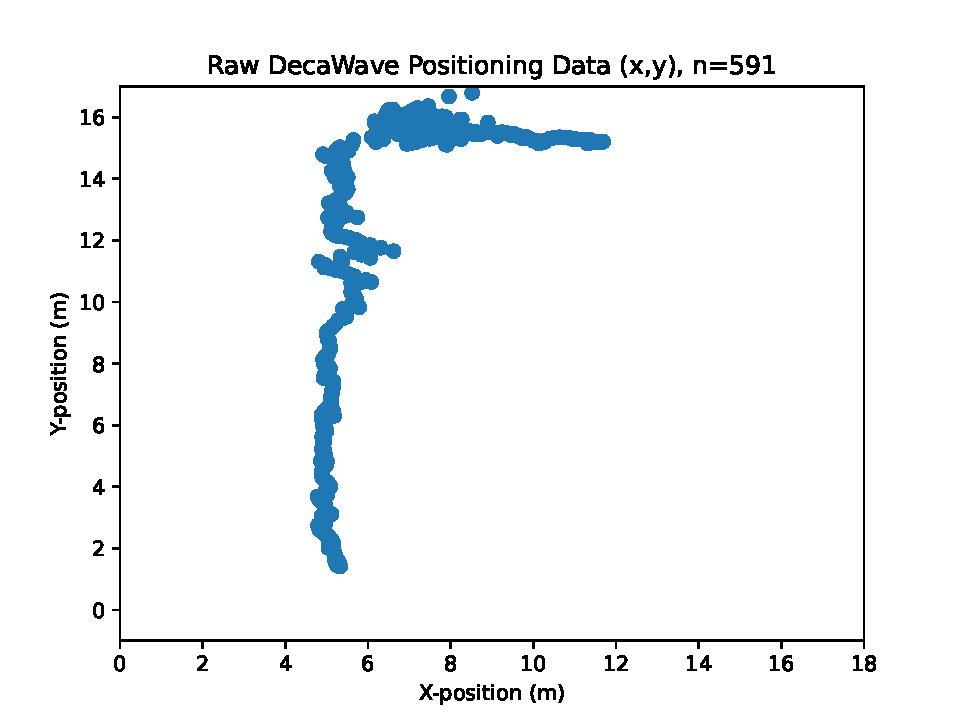
\includegraphics[width=\linewidth]{./images/test1_decawave.pdf}
         \caption{Test 1 -- a representative example.}
         \label{figure:test1_decawave}
%     \hfill
%     \begin{subfigure}[b]{0.49\textwidth}
%         \centering
%         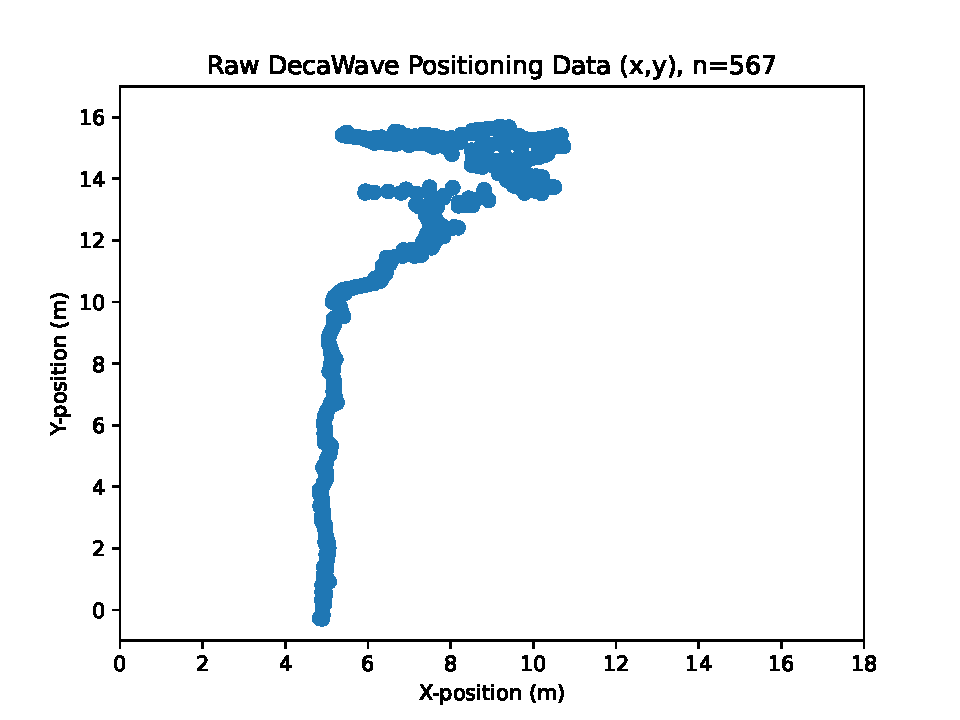
\includegraphics[width=\textwidth]{./images/test2_decawave.pdf}
%         \caption{Test 2}
%         \label{figure:test2_decawave}
%     \end{subfigure}
%     \hfill
%     \begin{subfigure}[b]{0.49\textwidth}
%         \centering
%         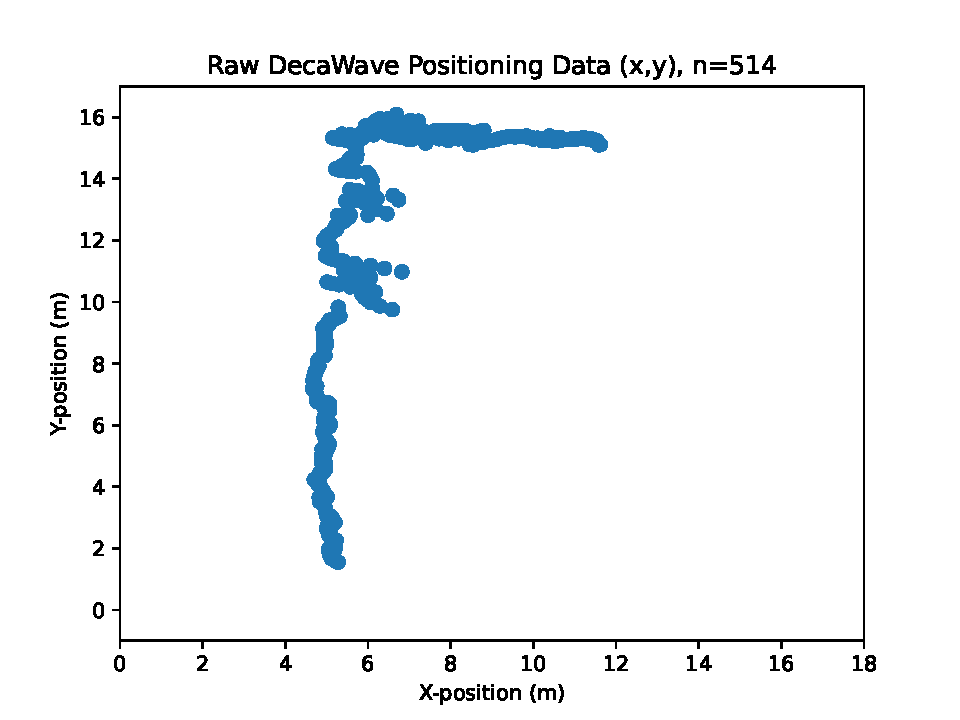
\includegraphics[width=\textwidth]{./images/test3_decawave.pdf}
%         \caption{Test 3}
%         \label{figure:test3_decawave}
%     \end{subfigure}
%        \caption{The raw DecaWave data visualized.}
%        \label{figure:decawave123_raw}
\end{figure}

\subsection{Heading Estimation}

Figures~\ref{figure:test1_yaw}, \ref{figure:test2_yaw}, and~\ref{figure:test1_yaw} show the
angular velocity measured by the gyroscope,
as well as the smoothed angular velocity and estimated angular position as measured by the Kalman Filter.
Figure~\ref{figure:test1_yaw} correctly shows a clockwise turn of $90^\circ \approx 1.578 \text{ rad}$.
Figure~\ref{figure:test2_yaw} correctly shows the opposite -- a counter-clockwise turn of
$-90^\circ \approx -1.578 \text{ rad}$.
Figure~\ref{figure:test3_yaw} shows a seemingly erroneous clockwise turn of about $45^\circ \approx 0.79\text{ rad}$, which needs investigation.

The \texttt{filterpy} implementation of the Kalman filter behaves badly (giving no output),
if the value for $d_t$ is adjusted at each timestep in $F$,
and I therefore had to use only a constant 0.067s.
Thinking that this could be an explanation for the inaccuracy in Figure~\ref{figure:test3_yaw},
I analyzed the \emph{actual} difference in time between frames for mean and standard deviation,
as in Table~\ref{table:dt_statistical_values}.
However, this shows that Test 3 actually has medium values for both mean and stddev.
The fact that Tests 2 and 3 have the most different values for mean and stddev mean
that inconsistency in $d_t$ should be more likely to major differences in performance.

\begin{table}
	\centering
	\begin{tabular}{|l|c|c|}
		\hline
		Test & $\mu_{d_t}$ & $\sigma_{d_t}$ \\\hline
		Test 1 & 0.0704 & 0.0209 \\\hline
		Test 2 & 0.0822 & 0.0405 \\\hline
		Test 3 & 0.0776 & 0.0360 \\\hline
	\end{tabular}
	\caption{Statistical values for actual $d_t$ in each test case.}
	\label{table:dt_statistical_values}
\end{table}

\begin{figure}
	\centering
	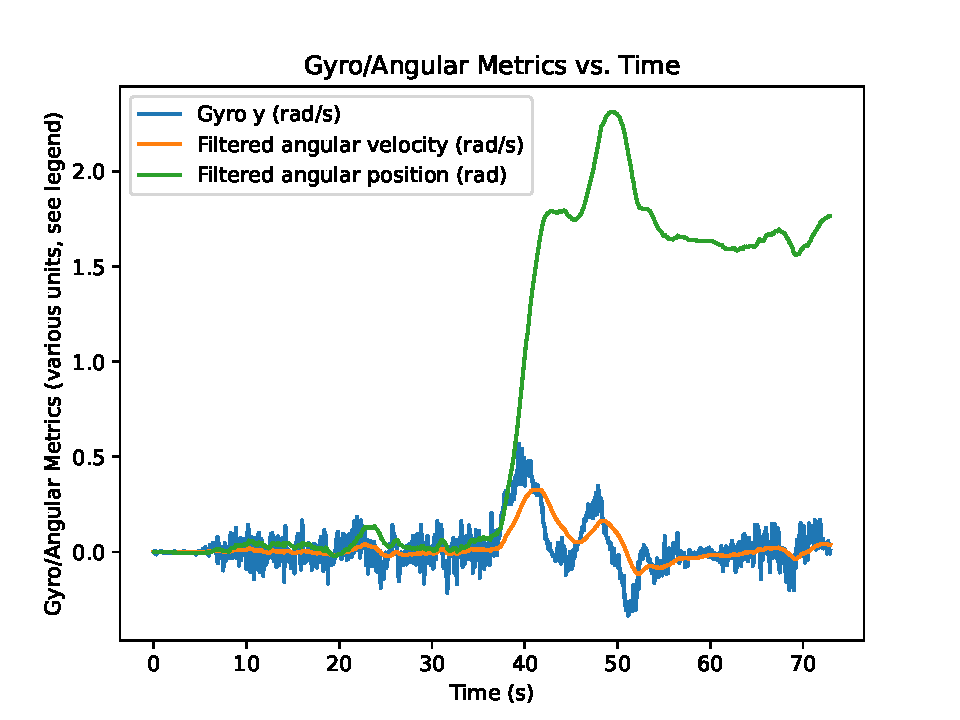
\includegraphics[width=\linewidth]{./images/test1_yaw.pdf}
	\caption{Heading for test 1, with raw gyro data (angular velocity), and angular velocity and position as estimated by the Kalman filter.}
	\label{figure:test1_yaw}
\end{figure}

\begin{figure}
	\centering
	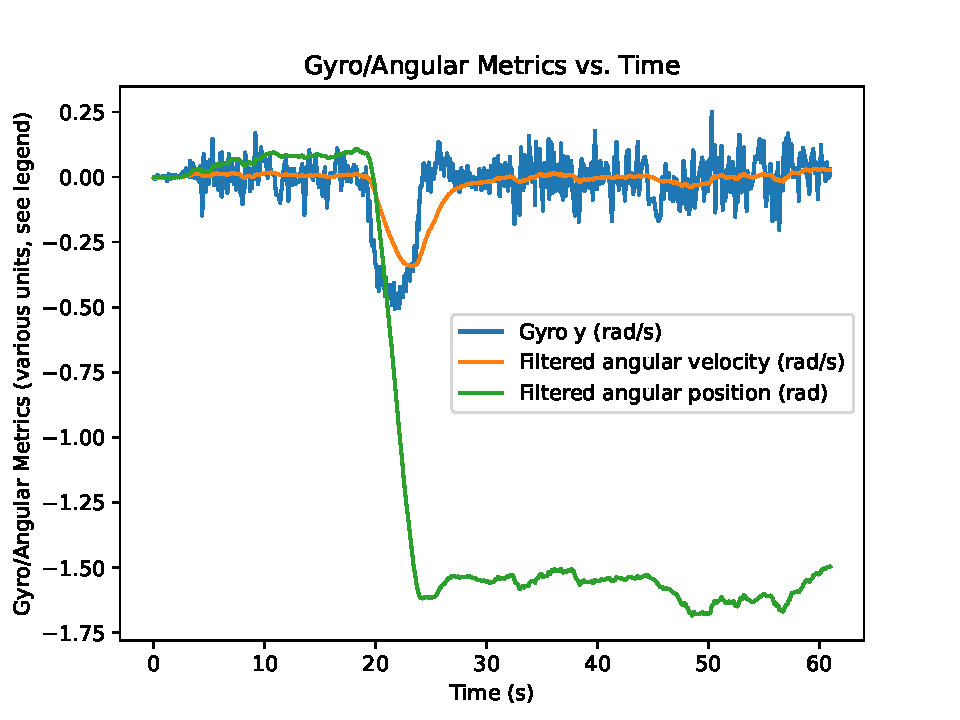
\includegraphics[width=\linewidth]{./images/test2_yaw.pdf}
	\caption{Heading for test 2, with raw gyro data (angular velocity), and angular velocity and position as estimated by the Kalman filter.}
	\label{figure:test2_yaw}
\end{figure}

\begin{figure}
	\centering
	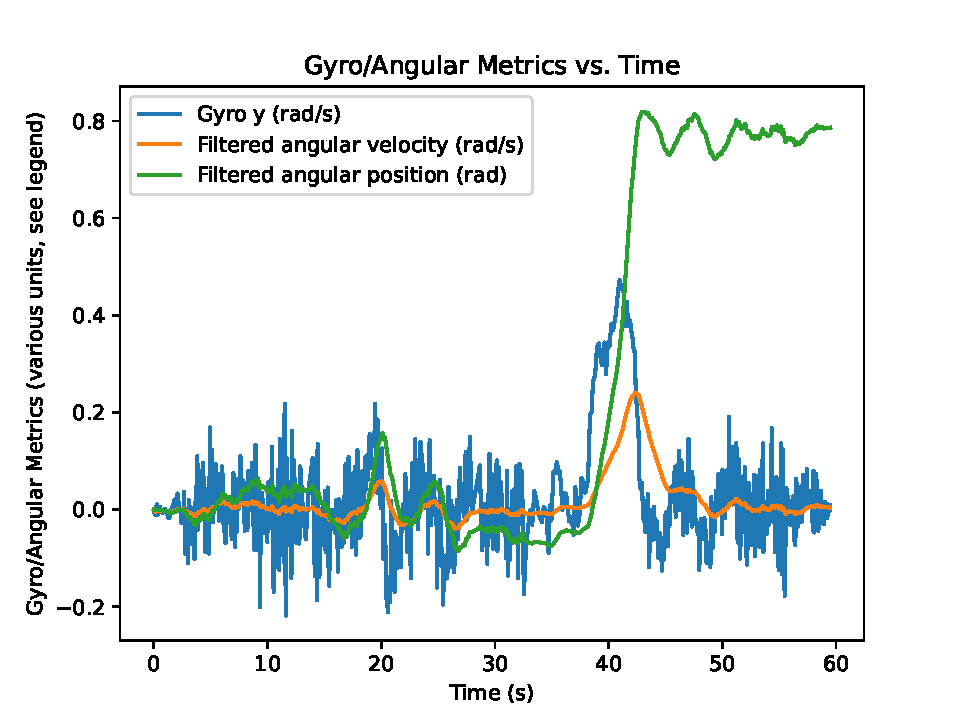
\includegraphics[width=\linewidth]{./images/test3_yaw.pdf}
	\caption{Heading for test 3, with raw gyro data (angular velocity), and angular velocity and position as estimated by the Kalman filter.}
	\label{figure:test3_yaw}
\end{figure}

\subsection{Depth Flow Velocity Estimation}

Figure~\ref{figure:depth_flow123_raw} shows the raw depth flow data (forward velocity only).
Unfortunately it seems that the changing scenery has decreased the usefulness of this data.
The velocity estimate depends on pixels mostly belonging to the same objects over time,
which was the case during the initial tests, where the drone was only moving forward and backward
over a small range (with no rotation) facing a wall that was far away.
In these test cases, the drone had nearby obstacles close to its left and right sides,
and as it moved past them, they had a high pixel velocity in the x-direction,
which is one factor in the noisy, unreliable data.

\begin{figure}
	\centering
		\centering
		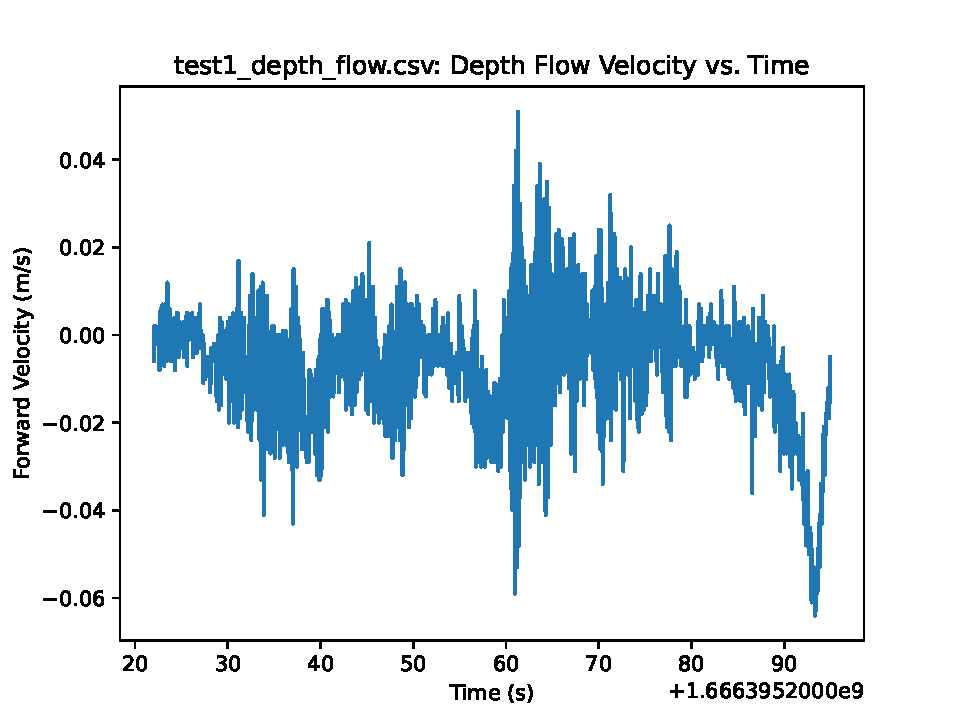
\includegraphics[width=\linewidth]{./images/test1_depth_flow_depth_forward_velocity.pdf}
		\label{figure:test1_depth_flow}
	\caption{The raw depth flow data visualized for Test Case 1 -- a representative example.}
	\label{figure:depth_flow123_raw}
\end{figure}

\subsection{Filtering Methods}

I have plotted the raw, filtered, and ground truth values from the DecaWave experiments
in Figure~\ref{figure:test3_decawave_and_ground_truth}.
%\ref{figure:test2_decawave_and_ground_truth},
%and~\ref{figure:test3_decawave_and_ground_truth}.
\begin{figure}
	\centering
	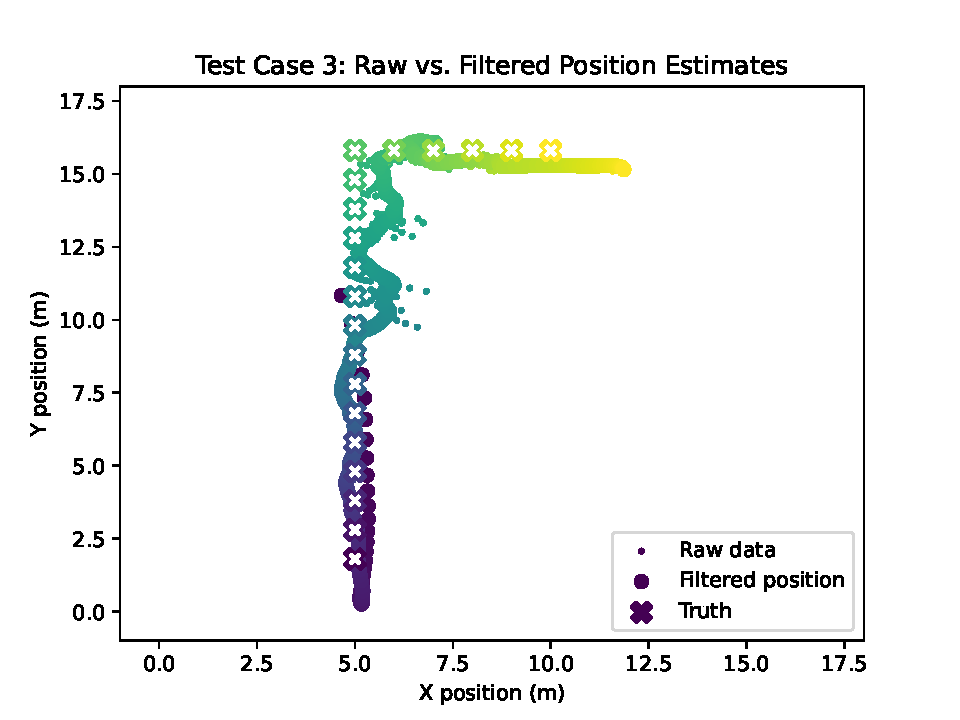
\includegraphics[width=\linewidth]{./images/test3_decawave_and_ground_truth.pdf}
	\caption{The raw, filtered, and ground truth values for the DecaWave system in Test Case 3.}
	\label{figure:test3_decawave_and_ground_truth}
\end{figure}
They are organized by color, such that the most purple points are the oldest and occurred at the
start of the experiment, and the most yellow points are the newest and occurred at the end of the
experiment.
The small points (sometimes obscured) represent the raw data,
the larger points represent the filtered data,
and the Xs represent the ground truth.
Each of the systems' begin at an assumed position of $(0,0)$,
leading to the curved, extraneous purple tail in all of the test cases.

Figure~\ref{figure:particle_filter_1} shows the performance of the 2-dimensional particle filter on the
raw DecaWave data.

\begin{figure}
	\center
	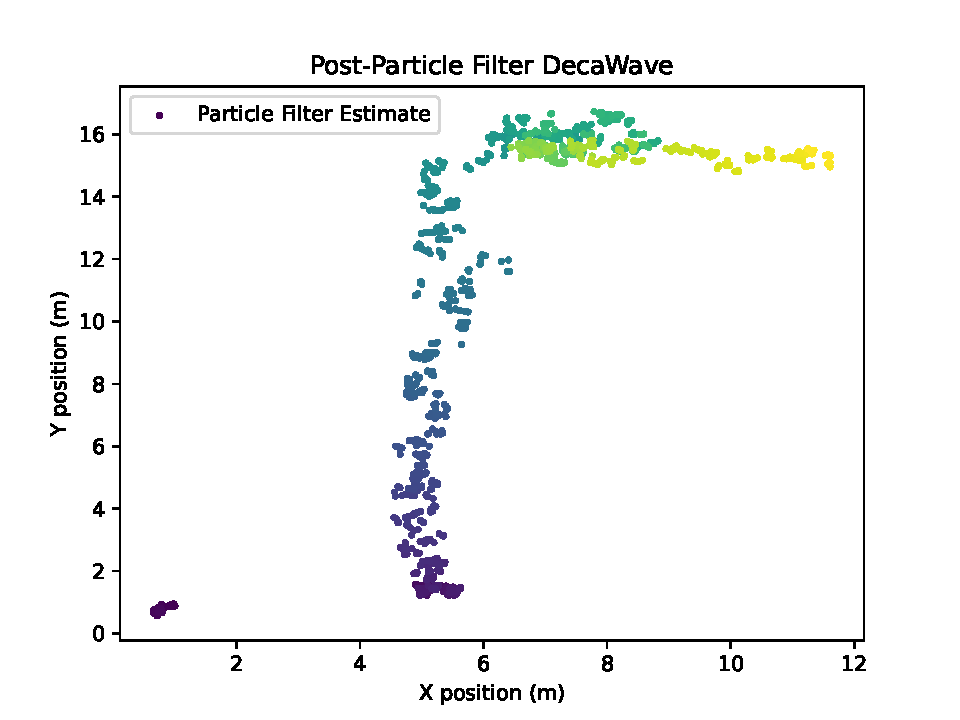
\includegraphics[width=\linewidth]{./images/particle_filter_test1.pdf}
	\caption{Particle filter visualization for Test Case 1}
	\label{figure:particle_filter_1}
\end{figure}

\subsection{Error Rates}

Table~\ref{table:error_rates} shows the error rates for each of the working systems.
The raw DecaWave did not have the best (lowest) error in any test case, no system outperformed
both competitors in all cases.
The particle filter gives the lowest error in test case 1, and the Kalman filter gives the lowest
error in the other test cases.

\begin{table}
	\centering
	\begin{tabular}{|l|c|c|c|}
	\hline
			& DecaWave & DecaWave + Kalman Filter & DecaWave + Particle Filter \\\hline
	Test Case 1 	& 0.6000 & 0.6562 & 0.4080 \\\hline
	Test Case 2	& 2.4653 & 2.3597 & 1.4205 \\\hline
	Test Case 3	& 0.7304 & 0.7040 & 0.9668 \\\hline
	\end{tabular}
	\caption{The average errors (m) of each system in each test case.}
	\label{table:error_rates}
\end{table}

%\begin{figure}
%	\centering
%	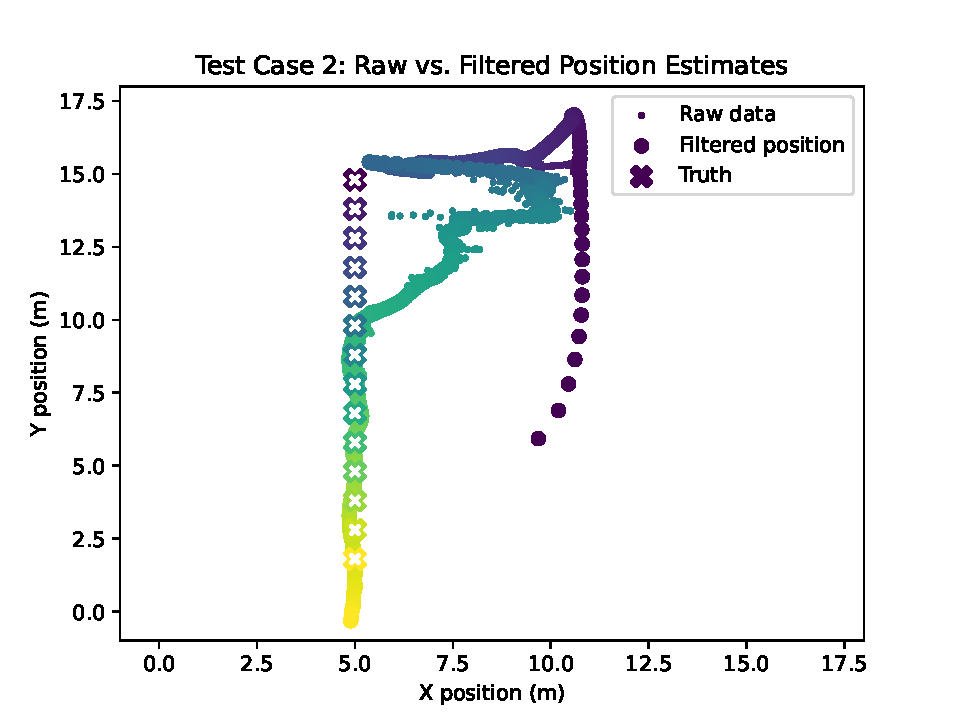
\includegraphics[width=0.8\textwidth]{./images/test2_decawave_and_ground_truth.pdf}
%	\caption{The raw, filtered, and ground truth values for the DecaWave system in Test Case 2.}
%	\label{figure:test2_decawave_and_ground_truth}
%\end{figure}

